
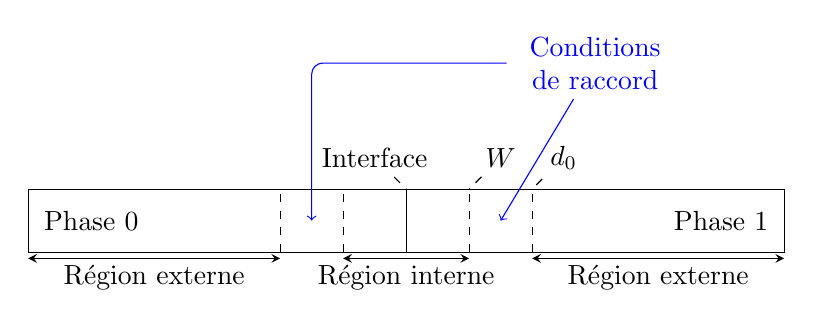
\begin{tikzpicture}[x={(0.8cm,0cm)}, y={(0cm,0.8cm)}, z={(-3.85mm, -3.85mm)}]
%styledesnœuds
\tikzstyle{textLine}=[rectangle, text=black]
\tikzstyle{textw}=[rectangle, text=black]
%figure
\draw (-6,0) rectangle + (12,1);
\draw[dashed] (-2,0) -- (-2,1);% d0 min
\draw[dashed] (-1,0) -- (-1,1);% W min

\node[textLine] (W) at (1.5,1.5) {$W$};
\draw[dashed] (W) -- (1,1);
\draw[dashed] (1,0) -- (1,1);  % W max

\node[textLine] (d0) at (2.5,1.5) {$d_0$};
\draw[dashed] (d0) -- (2,1);
\draw[dashed] (2,0) -- (2,1);  % d0 max
% interface
\draw[] (0,0) -- (0,1); 
\node[textLine] (interface) at (-0.5,1.5) {Interface};
\draw[dashed] (interface) -- (0,1);
%text
\node[textLine] (solide) at (-5,0.5) { Phase 0 };
\node[textLine] (liquide) at (5,0.5) { Phase 1 };
%vecteur
\tikzstyle{vector}=[->,thin,rounded corners=4pt]

% inner
\draw[stealth-stealth,thin] (-1,-0.1) -- (1,-0.1);
\node[textLine] (W) at (0,-0.4) {Région interne};

% outer
\draw[stealth-stealth,thin] (-6,-0.1) -- (-2,-0.1);
\draw[stealth-stealth,thin] (2,-0.1) -- (6,-0.1);
\node[textLine] (ext) at (4,-0.4) {Région externe};
\node[textLine] (ext) at (-4,-0.4) {Région externe};
% \node[textLine] (ext) at (3,-1.5) {Outer domain};
% \draw[vector] (ext) -- (-3,-1.5) -- (-3,-0.1);
% \draw[vector] (ext) -- (3,-0.1);

%match
\node[textLine, text width=2cm, text centered, color=blue] (cdt) at (3,3) {Conditions de raccord};
\draw[vector, color=blue] (cdt) -- (1.5,0.5);
\draw[vector, color=blue] (cdt) --(-1.5,3)-- (-1.5,0.5);
\end{tikzpicture}
